\section{Beehive server}

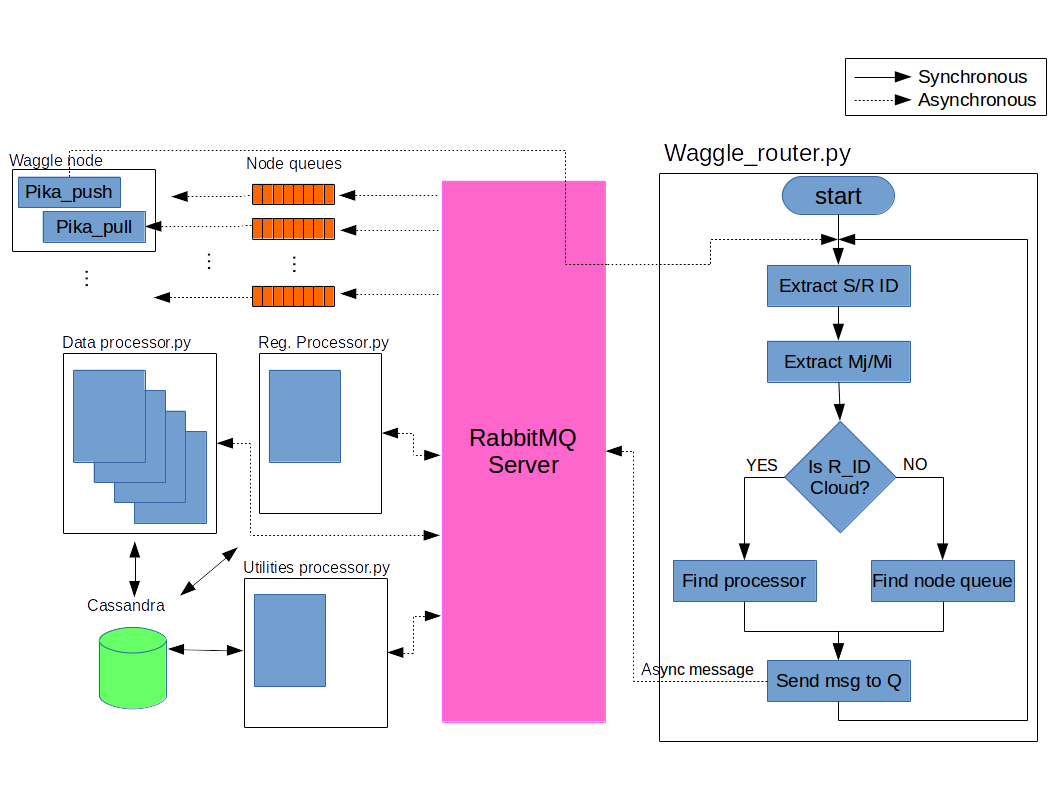
\includegraphics[width=\textwidth]{beehive_diagram.png}

\subsection{Store data}

After unpacking Waggle message, the actual payload message is JSON type. Server process should handle JSON data to pull values and store them in the database. 
JSON data consist of the following format. for now the format is based on `sensor\_table' scheme.

\begin{framed}
\noindent
node\_id, date, plugin\_id, plugin\_version, plugin\_instance, timestamp, sensor, sensor\_meta, data
\end{framed}

\textbf{TODO: Do we need to look up the routing table in the server everytime when a Waggle message comes to the 
server?}